\documentclass[11pt]{beamer}
\usetheme{CambridgeUS}
\usepackage[utf8]{inputenc}
\usepackage{amsmath}
\usepackage{amsfonts}
\usepackage{amssymb}
\usepackage{graphicx}
\usepackage{pgfpages}
\usepackage{framed}
\usepackage{xcolor}
\usepackage[most]{tcolorbox}
\usepackage{soul}
\usepackage{empheq}
\usepackage{minted}

% The replacement character � (often displayed as a black rhombus with a white
% question mark) is a symbol found in the Unicode standard at code point U
% +FFFD in the Specials table. It is used to indicate problems when a system 
% is unable to render a stream of data to a correct symbol.[4] It is usually 
% seen when the data is invalid and does not match any character. For this 
% reason we map explicitly this character to a blanck space.
\DeclareUnicodeCharacter{FFFD}{ }

\newcommand*{\itemimg}[1]{%
  \raisebox{-.3\baselineskip}{%
    \includegraphics[
      height=\baselineskip,
      width=\baselineskip,
      keepaspectratio,
    ]{#1}%
  }%
}

\newtcbox{\mymath}[1][]{%
    nobeforeafter, math upper, tcbox raise base,
    enhanced, colframe=blue!30!black,
    colback=blue!10, boxrule=1pt,
    #1}

\newcommand{\highlight}[1]{%
  \colorbox{yellow!50}{$\displaystyle#1$}}

\author{Giovanni Della Lunga\\{\footnotesize giovanni.dellalunga@unibo.it}}
%\title{2.1 - Data Pre-Processing}
%\title{4.1 - Linear and Logistic Regression}
%\title{4.2 - Decision Trees}
\title{Deep Learning Derivatives Pricing}
%\title{5 - Introduction to Reinforcement Learning}
\subtitle{} % (optional)
\setbeamercovered{transparent} 
\institute{Advanced Machine Learning for Finance} 
\date{Bologna - April-May, 2022} 

\begin{document}

%\begin{frame}
%\includegraphics[width=\linewidth]{img/halloween-seminar-logo.PNG}
%\end{frame}

\begin{frame}
\titlepage
\end{frame}

\AtBeginSection[]
{
  %\begin{frame}<beamer>
  %\footnotesize	
  %\frametitle{Outline}
  %\begin{multicols}{2}
  %\tableofcontents[currentsection]
  %\end{multicols}	  
  %\normalsize
  %\end{frame}
  \begin{frame}
  \vfill
  \centering
  \begin{beamercolorbox}[sep=8pt,center,shadow=true,rounded=true]{title}  	\usebeamerfont{title}\insertsectionhead\par%
  \end{beamercolorbox}
  \vfill
  \end{frame}
}

\AtBeginSubsection{\frame{\subsectionpage}}

% INSERT HERE

%---------------------------------------------------------------------------------------------------
\section{The Option Pricing Problem}
%---------------------------------------------------------------------------------------------------

\begin{frame}{Call and Put Options}
\begin{itemize}
\item Call option is an option to buy an asset on a certain future date (the maturity) for a certain price (the strike price)
\item Put option is an option to sell an asset on a certain future date (the maturity) for a certain price (the strike price)
\end{itemize}
\end{frame}
%..................................................................
\begin{frame}{The Payoffs}
	 
	\begin{center}
	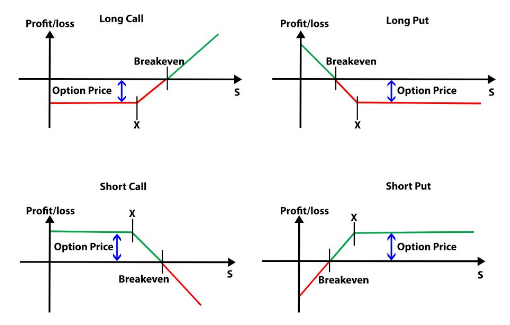
\includegraphics[scale=0.75]{../5-pictures/chapter-2_pic_0.png}
	\end{center}
\end{frame}
%..................................................................
\begin{frame}{Importance of volatility}
The asymmetry in the payoff means that volatility, $\sigma$,  is important in determining option prices. As volatility increases, the price of a call or put option increases. 
	\begin{center}
	\includegraphics[scale=0.5]{../5-pictures/chapter-4_pic_0.png}
	\end{center}

\end{frame}
%..................................................................
\begin{frame}{Moneyness}
	\begin{itemize}
		\item Moneyness is a measure of the extent to which an option is likely to be exercised
		\item Popular definitions (S = asset price, K = strike price)
		\item At-the money: $S = K$
		\item In-the money: $S > K$ for call options and $S<K$ for put options
		\item Out-of-the-money: $S<K$ for call options and $S>K$  for put options
	\end{itemize}
\end{frame}
%..................................................................
\begin{frame}{Implied volatilities}
\begin{itemize}
\item The Black-Scholes-Merton price of an option depends on $S, K, r, q, \sigma$,  and $T$.
\item $S, K$, and $T$ are known for an option
$r$ and $q$ can be estimated from futures or forward contracts
\item This means that $\sigma$ is the only unknown.
\item There is a one-to-one correspondence between option price and $\sigma$
\item The implied volatility of an option is the volatility that when substituted into Black-Scholes-Merton formula gives the price of the option in the market
\end{itemize}
\end{frame}
%..................................................................
\begin{frame}{Implied volatilities (continued)}
	\begin{itemize}
		\item If Black-Scholes-Merton was used for pricing, all options on an asset would have the same implied volatility
		\item In fact, there is quite a variation in implied volatilities
		\item Nevertheless implied volatilities are used to communicate prices and it is therefore important for traders to monitor implied volatilities
		\item The volatility surface shows implied volatilities as a function of Moneyness (measured by delta) and Time to maturity, T
	\end{itemize}
\end{frame}
%..................................................................
\begin{frame}{Volatility Surfaces for S\&P 500 }
	\begin{center}
	\includegraphics[scale=0.6]{../5-pictures/chapter-4_pic_0.png}
	\end{center}
\end{frame}
%..................................................................
\begin{frame}{Option Pricing Models}
Why we need option pricing models?
	\begin{itemize}
		\item Not all plain vanilla options listed on the market are sufficient for customer needs;
		\item \textbf{exotic options} are generally not as actively traded as plain vanilla options
		\item As a result, a
model is required for pricing;
\item A variety of different models are used in practice.
	\end{itemize}
\end{frame}
%..................................................................
\begin{frame}{Option Pricing Models}
Two conditions that traders would like the model to satisfy are:

	\begin{itemize}
\item (A) The stochastic behavior assumed for the underlying asset price should correspond reasonably well to its observed behavior, and

\item (B) The volatility surface derived from the model should be reasonably consistent with the volatility surface used to price plain vanilla options.
	\end{itemize}
\end{frame}
%..................................................................
\begin{frame}{Option Pricing Models}
	\begin{itemize}
\item	Two categories of models that are used in practice can be distinguished. 
\item The models in the first category focus on condition (A) by assuming a process for the asset price that is roughly consistent with its observed behavior. 
\item The models have parameters that can be chosen to provide an
approximate fit to the current volatility surface. 
\item Models in the second category focus on condition (B)
and are designed to be exactly consistent with the current volatility surface.
	\end{itemize}
\end{frame}
%..................................................................
\begin{frame}{Option Pricing Models}
	\begin{itemize}
		\item The usual approach to implementing models in the first category is to choose model
parameters to fit the volatility surface as closely as possible. 
\item This approach, which we refer to as
the \textbf{model calibration approach} or \textbf{MCA}. 
\item A drawback of the approach is that some of the points on the volatility
surface are likely to be more important than others for any particular exotic option that is
considered. 
\item It is of course possible to vary the weights assigned to different points on the volatility
surface according to the instrument being valued. 
\item However, it is difficult to determine in advance
what these weights should be, as a result, the points are usually given equal weight when model
parameters are determined.

	\end{itemize}
\end{frame}

%---------------------------------------------------------------------------------------------------
\section{Deep Learning Option Pricing}
%---------------------------------------------------------------------------------------------------
%..................................................................
\begin{frame}{Deep Learning Option Pricing}
	\begin{itemize}
		\item A model is essentially a sort of complex mapping from a set of parameters to the market price;
		\item Let's say, from a very general point of view, that we have a contingent claim $\cal{V}$ that depends on $D$ parameters:

$$
{\cal{V}}(\mathbf{x}), \, \mathbf{x}=\left\{x_1,\dots, x_D \right\} \in \mathbb{R}^D
$$

\item We want to \textbf{approximate the pricing function with a neural network}. 
\item Remember that we can always consider the NN as a sort of mapping function 

$$
\Phi : \mathbb{R}^D \rightarrow \mathbb{R}
$$

trained to compute prices given a point in $\mathbb{R}^D $ representing a particular set of parameters.  
	\end{itemize}
\end{frame}
%..................................................................
\begin{frame}{Deep Learning Option Pricing}
	\begin{itemize}
		\item The use of a NN as a pricing functions has a number of advantages. 
		\item The first is that in this way we are able to compute efficiently thousands of prices in a small amount of time, even when the derivative contract has complicated conditions and when the model is complex. 
		\item This comes with the downside that the neural network \textbf{may introduce systematic errors} that could affect our estimation of the sensitivities in a number of ways. 

	\end{itemize}
\end{frame}
%..................................................................
\begin{frame}{Deep Learning Option Pricing}
	\begin{itemize}
		\item The second advantage is that instead of training the network on the model parameters, which in general are not observable, we could train the network \textbf{using data that is directly observable in the market}. 
		\item For example quotes and trades by market participants provide points on the
volatility surface. 
\item Interpolating between these points as necessary, a trader can derive a reasonable
estimate of the implied volatility appropriate for any new plain vanilla European or American option that is of interest. 
\item The volatility surface derived from the Black–Scholes–Merton model is a convenient interpolation tool for doing this.

	\end{itemize}
\end{frame}
%..................................................................
\begin{frame}{Deep Learning Option Pricing}
This allows us to define a new type of pricing approach. We refer to this approach as the \textbf{volatility feature approach} or \textbf{VFA}.
	\begin{itemize}
		\item We create a neural
network where the inputs are \textbf{the volatility surface points} and \textbf{the exotic option parameters} and \textbf{the
target is the price}. 
\item We randomly generate many sets of parameters for (a) the model under
consideration and (b) the exotic option under consideration. 
\item For each set of parameters, a volatility
surface and a price for the exotic option are calculated. 
\item The neural network is then constructed.
	\end{itemize}
The model parameters are used to create the training set, but \textbf{they are not inputs to the neural network}.
\end{frame}
%..................................................................
\begin{frame}{Deep Learning Option Pricing}
\begin{center}
\includegraphics[scale=.7]{../5-pictures/chapter-2_pic_3.png} 
\end{center}
\end{frame}
%..................................................................
\begin{frame}{Deep Learning Option Pricing}
\begin{center}
\includegraphics[scale=.7]{../5-pictures/chapter-2_pic_4.png} 
\end{center}
\end{frame}
%..................................................................
\begin{frame}{Deep Learning Option Pricing}
	\begin{itemize}
		\item The VFA approach is a compromise between models that satisfy condition (A) and those that
satisfy condition (B). 
\item It retains some of the structure of an analyst’s preferred model while learning
which points on the volatility surface are most important for the exotic option being valued. 
\item The idea behind
this method is that by sampling the volatility smile with enough points one
should be able to obtain all the informations that would be contained in the
model parameters, which is an assumption already implicitly made by market
practitioners when they calibrate their model parameters on the volatility
smile.
\item For this reason, it produces prices for exotic options that are more consistent with the prices of vanilla options than MCA.
	\end{itemize}
\end{frame}
%..................................................................
\begin{frame}{Deep Learning Option Pricing}
Let's call $\Pi( \vec{\alpha}, G(\vec{g}) )$ the function pricing a position $G$ with a model described
collectively by the parameters $\vec{\alpha}$, and the position described by the parameters $\vec{g}$. To be clear, in case of an option $\vec{g}$ could be the the pair maturity and strike. 

A standard ML exercise would call for 
	\begin{itemize}
		\item generating, according to some random rule, a set of parameters $\vec{\alpha}_n,\; \vec{g}_n\; 1 \le n \le N$
\item for each $\vec{\alpha}_n\, \vec{g}_n$ compute the function pricing a derivative $G$ with a model described by the parameter set $\vec{\alpha}_n$. We define the total parameter set as  $\Pi_n := \Pi( \vec{\alpha}_n, G(\vec{g}_n))$
 
	\end{itemize}
\end{frame}
%..................................................................
\begin{frame}{Deep Learning Option Pricing}
Iterating the procedure described above, we can build a large matrix 
		\begin{center}
	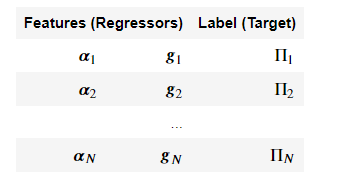
\includegraphics[scale=0.75]{../5-pictures/chapter-2-temp_pic_1.png}
		\end{center}
and use it to train a neural network that, if all goes well, will learn the map
\begin{equation}
    \phi_{NN}: \vec{\alpha}, \vec{g} \rightarrow \Pi(\vec{\alpha}, G).
\end{equation}     
\end{frame}
%..................................................................
%---------------------------------------------------------------------------------------------------
\section{A Worked Example}
%---------------------------------------------------------------------------------------------------
%..................................................................
\begin{frame}{Working Path}
During these lessons we will develop the approach described through 3 examples: 
	\begin{itemize}
		\item Description of the training process of a network using the Black and Scholes model; 
		\item Training of a stochastic volatility model (Heston) starting from the data of the model itself (MCA) and ...
		\item Training of a model starting from market data (volatility surface) following the VFA approach;
	\end{itemize}
	
The network will be trained on a large synthetic dataset generated by
drawing each parameter from an appropriate distribution and by calculating
the corresponding exact vanilla option price (and the implied volatility surface for the last example).	The parameter's sampling will be done using the \textbf{Latin Hypercube Sampling (LHS)} approach.
\end{frame}
%..................................................................
\begin{frame}{Creation of the synthetic sets}
\textbf{What is Latin Hypercube Sampling?}
\begin{itemize}
\item Latin hypercube sampling is a method that can be used to sample random numbers in which samples are distributed evenly over a sample space.

\item The idea behind one-dimensional latin hypercube sampling is simple: Divide a given CDF into $n$ different regions and randomly choose one value from each region to obtain a sample of size $n$.
\item It is a sort of \textbf{stratified sampling}

\item The benefit of this approach is that \textbf{it ensures that at least one value from each region is included in the sample}.
\end{itemize}
\end{frame}
%..................................................................
\begin{frame}{Creation of the synthetic sets}
\textbf{What is Latin Hypercube Sampling?}
\begin{itemize}
\item Suppose we’d like to obtain a sample of 2 values from a dataset that is normally distributed with a mean of 0 and a standard deviation of 1.

\item If we used a simple random number generator to obtain this sample, it’s possible that both values could be greater than 0 or that both values could be less than 0.

\item However, if we used latin hypercube sampling to obtain this sample then it would be guaranteed that one value would be above 0 and one would be below 0 because we could specifically partition the sample space into one region with values above 0 and one region with values below 0, then select a random sample from each region.
\end{itemize}
\end{frame}
%..................................................................
\begin{frame}{Creation of the synthetic sets}
\textbf{What is Latin Hypercube Sampling?}
\begin{itemize}
\item We can easily extend the idea of one-dimensional latin hypercube sampling into two dimensions as well.

\item For two variables, $x$ and $y$, we can divide the sample space of each variable into  $n$ evenly spaced regions and pick a random sample from each sample space to obtain random values across two dimensions.
\end{itemize}
	\begin{center}
	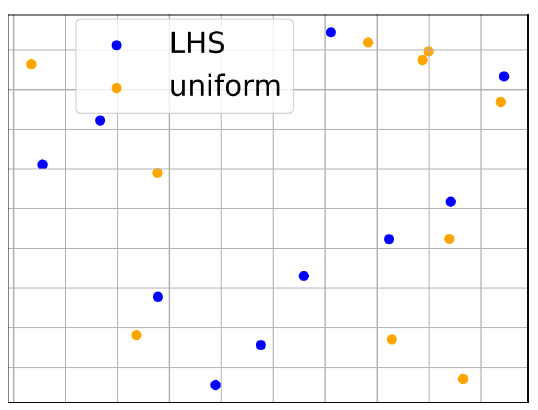
\includegraphics[scale=.175]{../5-pictures/chapter-2-temp_pic_3.png}
	\end{center}
\end{frame}
%..................................................................
\begin{frame}{Creation of the synthetic sets}
\textbf{What is Latin Hypercube Sampling?}
\begin{itemize}
\item To perform latin hypercube sampling in greater dimensions, we can simply extend the idea of two-dimensional latin hypercube sampling into even more dimensions.

\item Each variable is simply split into evenly spaced regions and random samples are then chosen from each region to obtain a controlled random sample.

\item The main advantage of latin hypercube sampling is that it produces samples that reflect the true underlying distribution and it tends to require much smaller sample sizes than simple random sampling. 

\item This method of sampling can be particularly advantageous if you’re working with data that has a high number of dimensions and you need to obtain random samples that are sure to reflect the true underlying distribution of the data.
\end{itemize}
\end{frame}
%..................................................................
\begin{frame}[fragile]
\frametitle{Creation of the synthetic sets}
\begin{itemize}
		\item To train the network to approximate the pricing function, we need a training
dataset. 
\item For the network approximating the Black Scholes pricing function,
we created one by drawing $T$, $K/S_0$ and $\sigma$ using LHS (Latin Hypercube Sampling) within the ranges
usually found in real market.
\end{itemize}
\rule{\textwidth}{1pt}
\scriptsize
\begin{minted}{python}

# Lower and upper boundaries for each parameter
bounds = {  "T"     : [1./12., 2.00]
          , "Sigma" : [ .01  ,  .80]
          , "Strike": [ .4   , 1.20]
         }
# Number of Observations
NUM = 100000
# Random number generator
rand = np.random.RandomState(42)
# Latin Hypercube Sampling
xDF = lhs_sampling(rand, NUM, bounds=bounds)
xDF.head()

\end{minted}
\rule{\textwidth}{1pt}
\end{frame}
%..................................................................
\begin{frame}[fragile]
\frametitle{Creation of the synthetic sets}
\textbf{LHS Function Definition}
\rule{\textwidth}{1pt}
\scriptsize
\begin{minted}{python}

from smt.sampling_methods import LHS

def lhs_sampling(rand, NUM, bounds=None):
    mInt = 2**15
    MInt = 2**16
    kw   = list(bounds)
    # builds the array of bounds
    limits = np.empty(shape=(0,2))
    for k in kw: 
        limits = np.concatenate((limits, [bounds[k]]), axis=0)

    sampling = LHS(xlimits=limits, random_state=rand.randint(mInt,MInt))
    x        = sampling(NUM)
    X = pd.DataFrame()
    for n in range(len(kw)):
        tag    = kw[n]
        X[tag] = x[:,n]

    return X

\end{minted}
\rule{\textwidth}{1pt}
\end{frame}
%..................................................................
\begin{frame}[fragile]
\frametitle{Creation of the synthetic sets}
\textbf{Black and Scholes Price Generator}
\rule{\textwidth}{1pt}
\scriptsize
\begin{minted}{python}

def gen(NUM, lhs):
    x   = lhs
    __tStart = time.perf_counter()
    S0     = np.full(NUM, 1.0, dtype = np.double)
    r      = np.full(NUM, 0.0, dtype = np.double)
    price  = np_euro_call(S0, r, x["T"], x["Sigma"], x["Strike"])
    __tEnd = time.perf_counter()
    print("@ %-34s: elapsed %.4f sec" %("NP pricing", __tEnd-__tStart) )

    df = pd.DataFrame(x)
    df["Price"] = price

    return df

\end{minted}
\rule{\textwidth}{1pt}
\end{frame}
%..................................................................
\begin{frame}{Creation of the synthetic sets}
\begin{itemize}
\item As for the network approximating the pricing function in the Heston
model with the MCA approach, a synthetic set has been created by drawing Heston Model
parameters with LHS without accounting for the Feller condition.
\item We also trained a network to calculate the price of a vanilla put option in
the Heston model using the VFA approach with the contract parameters $T$
and $K/S_0$ and the implied volatility smile sampled on the 9 moneyness values
$K/S_0 \in \left\{0.4; 0.55; 0.7; 0.85; 1.0; 1.15; 1.3; 1.45; 1.6 \right\}$. 
\item The implied volatility
smiles are generated using the same parameters as those generated in the
dataset for the MCA.
\end{itemize}
\end{frame}
%..................................................................
\begin{frame}[fragile]
\frametitle{Creation of the synthetic sets}
\textbf{Heston Price Generator (MCA Approach)}
\rule{\textwidth}{1pt}
\scriptsize
\begin{minted}{python}

def parms_gen( lhs = None, Xc=10, strikes=None):
    x = lhs
    NUM = len(x["T"])
    for m in range(NUM):
        K     = x["Strike"][m]
        fwPut = HestonPut( St     = 1.0, Strike = K, T = x["T"][m]
                         , kappa  = x["k"][m], theta  = x["theta"][m]
                         , sigma  = x["sigma"][m], v0  = x["v0"][m]
                         , r      = 0, rho = x["rho"][m], Xc = Xc)
        for tag in list(x):
            X[tag][n] = x[tag][m]
        X["Price"][n] = fwPut
        n += 1
    df = pd.DataFrame()
    for s in X.keys(): df[s] = np.copy(X[s][0:nSamples])
    return df


\end{minted}
\rule{\textwidth}{1pt}
\end{frame}
%..................................................................
\begin{frame}[fragile]
\frametitle{Creation of the synthetic sets}
\textbf{Heston Price Generator (VFA Approach)}
\rule{\textwidth}{1pt}
\scriptsize
\begin{minted}{python}

def mkt_gen( lhs = None, kw = None, Xc=10, strikes=None):
	......................
    
    for m in range(NUM):
		
		..........	 
 
        fwPut = HestonPut(Fw, K, T, Kappa, Theta, sgma, Ro, Rho, 0.0, Xc)

        vol = build_smile(strikes, Fw, T, Kappa, Theta, sgma, Ro, Rho, Xc)

        for k in strikes:
            tag = "k=%5.3f" %k
            X[tag][n] = vol[tag]
        X["Price"][n]  = fwPut
        X["Strike"][n] = K
        X["T"][n]      = T

		..........

\end{minted}
\rule{\textwidth}{1pt}
\end{frame}
%..................................................................
\begin{frame}[fragile]
\frametitle{Creation of the synthetic sets}
\textbf{Heston Price Generator (VFA Approach)}
\rule{\textwidth}{1pt}
\scriptsize
\begin{minted}{python}

from Lib.euro_opt import impVolFromFwPut

def build_smile(strikes=None, Fw=1.0, T= 1.0, Kappa=1., 
                Theta=1., sgma=1.0, Ro=0.0, Rho=0.0, Xc=10):
    vol = {}
    for k in strikes:
        tag = "k=%5.3f" %k
        fwPut = HestonPut(Fw, k, T, Kappa, Theta, sgma, Ro, Rho, 0.0, Xc)
        if fwPut < max( k-Fw, 0.0): return None
        vol[tag] = impVolFromFwPut(price = fwPut, T = T, kT = k)

    return vol

\end{minted}
\rule{\textwidth}{1pt}
\end{frame}
%..................................................................
\begin{frame}{Network Architecture}
	\begin{itemize}
		\item All the neural networks used are composed of three dense layers of 200
neurons with 'relu' activations. 
\item For the neural network calculating the
vanilla option prices in the Black Scholes model, the features used are
the time to maturity $T$, the moneyness $K/S_0$ and the asset volatility $\sigma$.
\item For the network using the MCA approach to the Heston model the features
are the time to maturity $T$, the moneyness $K/S_0$ and the five model parameters
$\left\{ \kappa; \theta; \nu_0; \xi; \rho \right\}$.
\item For the network calculating the prices in the Heston model using the
VFA the features used are again the time to maturity $T$, the moneyness
$K/S_0$ and 9 samples of the implied volatility smile calculated in $K/S_0 \in \left\{0.4; 0.55; 0.7; 0.85; 1.0; 1.15; 1.3; 1.45; 1.6 \right\}$.
\end{itemize}
\end{frame}
%..................................................................
\begin{frame}[fragile]
\frametitle{Network Architecture}
\textbf{Black and Scholes Pricing Network}
\rule{\textwidth}{1pt}
\scriptsize
\begin{minted}{python}

def model_builder( inputShape = (1,)):
    model = Sequential()
    model.add(Dense(200, activation='relu', input_shape=inputShape))
    # Add one more hidden layer 
    model.add(Dense(200, activation='relu'))
    # Add one more hidden layer 
    model.add(Dense(200, activation='relu'))
    # Add an output layer 
    model.add(Dense(1))
    # Model output shape
    print("model.output_shape: %s" %(str(model.output_shape)))
    # Model summary
    print("Model.summary"); model.summary()
    # Model config
    print("Model.config"); model.get_config()
    model.compile(loss='mse', optimizer='rmsprop', metrics=['mae'])
    return model

\end{minted}
\rule{\textwidth}{1pt}
\end{frame}
%..................................................................
\begin{frame}{Let's code ...}
\begin{center}

\includegraphics[scale=.8]{../5-pictures/exercise.jpg} 
\end{center}
\end{frame}
%..................................................................
%---------------------------------------------------------------------------------------------------
\section{Understanding Volatility Surface Movements}
%---------------------------------------------------------------------------------------------------
%..................................................................
\begin{frame}{Volatility Surface Movements}
\begin{itemize}
\item When the price of the underlying asset increases (decreases), implied volatilities tend to decrease (increase)
\item However not all implied volatilities change by the same amount
\item This explains the variation in volatility surfaces
\end{itemize}
\end{frame}
%..................................................................
\begin{frame}{Volatility Surface Movements}
Understanding how the volatility surface moves is important
for a number of reasons:
	\begin{itemize}
		\item It can help a trader hedge her/his exposure;
		\item It can help a quant determine a stochastic volatility model reflecting
how options are priced in the market;
		\item It can help a trader adjust implied volatilities in a market where
asset prices are changing fast.
	\end{itemize}
\end{frame}
%..................................................................
\begin{frame}{Understanding Volatility Surface Movements}
To understand volatility surface movements we used data on S\&P 500 call options to construct a neural network
	\begin{itemize}
		\item \textbf{Input layer}:
		\begin{itemize}
		\item Daily asset price return
		\item Moneyness (measured by delta)
		\item Time to maturity
		\end{itemize}
		\item \textbf{Output layer}:
		\begin{itemize}
		\item Change in implied volatility
		\end{itemize}
	\end{itemize}
	The objective is to
minimize the mean squared error between the predicted change in the
implied volatility and the actual change.
\end{frame}
%..................................................................
\begin{frame}{Neural Network Architecture}
\begin{itemize}
\item 3 hidden layers
\item 20 neurons per layer
\item Observations from 2014-2019
\item Randomly sampled 100 options per day
\item 125700 options in total
\item 60\% for training set
\item 20\% for validation set
\item 20\% for test set
\item Z-score scaling
\end{itemize}
\end{frame}
%..................................................................
\begin{frame}[fragile]
\frametitle{Neural Network Architecture}
\rule{\textwidth}{1pt}
\scriptsize
\begin{minted}{python}
# Create ML Model
#
# Sequential function allows you to define your Neural Network in sequential 
# order. Within Sequential, use Dense function to define number of nodes, 
# activation function and other related parameters. For more information 
# regrading to activation function, please refer to 
#
# https://keras.io/activations/
#
model = keras.models.Sequential([Dense(20,activation = "sigmoid",
                                             input_shape = (3,))
                                ,Dense(20,activation = "sigmoid")
                                ,Dense(20,activation = "sigmoid")
                                ,Dense(1)])
# Model summary function shows what you created in the model
model.summary()
# Complie function allows you to choose your measure of loss and optimzer
# For other optimizer, please refer to https://keras.io/optimizers/
model.compile(loss = "mse",optimizer = "Adam")
\end{minted}
\rule{\textwidth}{1pt}
\end{frame}
%..................................................................
\begin{frame}{Benchmark Model}
\begin{itemize}
\item In constructing a machine learning model, it is always useful to have
a simpler model as a benchmark. In this case, we use the following model
\begin{equation}
\text{Expected Change in Implied Volatility} =R \frac{a+b\delta+c\delta^2}{\sqrt{T}}
\end{equation}
where $R$ is the return on the asset (= change in price divided by initial
price), $T$ is the option’s time to maturity, $\delta$ is the option’s moneyness
(measured as delta) and $a$, $b$, and $c$ are constants. 
\item This model was suggested
by Hull and White (2017) and is quite popular with practitioners.
\item The $a$, $b$, and $c$ can be estimated by regressing implied volatility changes
against $R/\sqrt{T}$, $R\delta/\sqrt{T}$, and $R\delta^2/\sqrt{T}$.
\end{itemize}
\end{frame}
%..................................................................
\begin{frame}[fragile]
\frametitle{Benchmark Model}
\textbf{Building variables for linear regression}
\rule{\textwidth}{1pt}
\scriptsize
\begin{minted}{python}

R     = raw['SPX Return']
RAD_T = np.sqrt(raw['Time to Maturity in Year'])
DELTA = raw['Delta']
# construct the 3 variables for regression
raw['x1'] = R / RAD_T
raw['x2'] = (R / RAD_T) * DELTA
raw['x3'] = (R / RAD_T) * DELTA * DELTA

# Put the X and Y variable in data frame for regression
y = raw['Implied Volatility Change']
X = raw[['x1', 'x2', 'x3','SPX Return','Time to Maturity in Year','Delta']]

\end{minted}
\rule{\textwidth}{1pt}
\end{frame}
%..................................................................
\begin{frame}[fragile]
\frametitle{Benchmark Model}
\textbf{Create training, test and validation set}
\rule{\textwidth}{1pt}
\scriptsize
\begin{minted}{python}

# Divide data into training set and test set(note that random seed is set)
X_train,X_test,y_train,y_test=train_test_split(  X
                                               , y
                                               , test_size    = 0.2
                                               , random_state = 100)

# Divide training set into training and validation set
X_train,X_val,y_train,y_val=train_test_split(  X_train
                                             , y_train
                                             , test_size    = 0.25
                                             , random_state = 100)
\end{minted}
\rule{\textwidth}{1pt}
\end{frame}
%..................................................................
\begin{frame}[fragile]
\frametitle{Benchmark Model}
\textbf{Run Regression}
\rule{\textwidth}{1pt}
\scriptsize
\begin{minted}{python}

# Run the regression on the training data
lr = LinearRegression(fit_intercept=False)
lr.fit(X_scaled_train[:,:3], y_train)

# Get the prediction
y_pred = lr.predict(X_scaled_test[:,:3])

# Calculate Mean Squared Error
mse = mean_squared_error(y_test, y_pred)

print('Test loss (MSE):', mse)

\end{minted}
\rule{\textwidth}{1pt}
\end{frame}
%..................................................................
\begin{frame}{Check-Point Deep Learning Models}
\begin{itemize}
\item Deep learning models can take hours, days or even weeks to train.
\item If the run is stopped unexpectedly, you can lose a lot of work.
\item You can check-point your deep learning models during training in Python using the Keras library.
\item A snapshot of the state of the system is taken in case of system failure. If there is a problem, not all is lost. 
\item The checkpoint may be used directly, or used as the starting point for a new run, picking up where it left off.
\end{itemize}
\end{frame}
%..................................................................
\begin{frame}{Check-Point Deep Learning Models}
\begin{itemize}
\item The ModelCheckpoint callback class allows you to define where to checkpoint the model weights, how the file should named and under what circumstances to make a checkpoint of the model.

\item The API allows you to specify which metric to monitor, such as loss or accuracy on the training or validation dataset. You can specify whether to look for an improvement in maximizing or minimizing the score. Finally, the filename that you use to store the weights can include variables like the epoch number or metric.

\item The ModelCheckpoint can then be passed to the training process when calling the fit() function on the model.

\item Note, you may need to install the h5py library to output network weights in HDF5 format.
\end{itemize}
\end{frame}
%..................................................................
\begin{frame}{Check-Point Deep Learning Models}
\begin{itemize}
\footnotesize
\item The Hierarchical Data Format version 5 (HDF5), is an open source file format that supports large, complex, heterogeneous data. 
\item HDF5 uses a "file directory" like structure that allows you to organize data within the file in many different structured ways, as you might do with files on your computer. 
\end{itemize}
\begin{center}
\includegraphics[scale=.175]{../5-pictures/hdf5_structure4.jpg} 
\end{center}
\end{frame}
%..................................................................
\begin{frame}[fragile]
\frametitle{Check-Point Deep Learning Models}
\scriptsize
\begin{itemize}
\item Checkpointing is setup to save the network weights only when there is an improvement in classification accuracy on the validation dataset (monitor=’val\textunderscore accuracy’ and mode=’max’).
\item The weights are stored in a file 'implied\textunderscore vol\textunderscore model\textunderscore vFinal.h5.h5'
\end{itemize}
\rule{\textwidth}{1pt}
\begin{minted}{python}

# Checkpoint function is used here to periodically save a copy of the model. 
# Currently it is set to save the best performing model
checkpoint_cb = keras.callbacks.ModelCheckpoint("implied_vol_model_vFinal.h5"
                                                , monitor='val_accuracy'
                                                , verbose=1
                                                , save_best_only=True
                                                , mode='max')

# Early stopping allows you to stop your training early if no improvment is 
# shown after certain period. Currently it is set at if no improvement 
# occured in 1000 epochs, at the stop the model will also revert back to 
# the best weight.
early_stopping_cb = keras.callbacks.EarlyStopping(patience = 1000

\end{minted}
\rule{\textwidth}{1pt}
\end{frame}
%..................................................................
\begin{frame}[fragile]
\frametitle{Train the Model}
\scriptsize
\rule{\textwidth}{1pt}
\begin{minted}{python}

# The fit function allows you to train a NN model. Here we have training data, 
# number of epochs,batch size, validation data, and callbacks as input
# Callback is an optional parameters that allow you to enable tricks for 
# training such as early stopping and checkpoint

# Remarks: Altough we put 50000 epochs here, the model will stop its training 
# once our early stopping criterion is triggered

history=model.fit(  X_scaled_train[:,3:6]
                  , y_train
                  , epochs=10
                  , batch_size = 128
                  , verbose = 1
                  , validation_data=(X_scaled_vals[:,3:6],y_val)
                  , callbacks=[checkpoint_cb, early_stopping_cb])

\end{minted}
\rule{\textwidth}{1pt}
\end{frame}
%..................................................................
\begin{frame}[fragile]
\frametitle{Train the Model}
\scriptsize
\rule{\textwidth}{1pt}
\begin{minted}{python}

# Load the best model you saved and calcuate MSE for testing set

model = keras.models.load_model("implied_vol_model_vFinal.h5")
mse_test = model.evaluate(X_scaled_test[:,3:6],y_test,verbose=0)

print('Test Loss(MSE):', mse_test)

# Calculate Gain Ratio

gain = 1 - mse_test/mse 

print('Gain Ratio:', gain)

\end{minted}
\rule{\textwidth}{1pt}
\end{frame}
%..................................................................
\begin{frame}{Mean Squared Error (Training stopped after 5,826 epochs)}
	 
	\begin{center}
	\includegraphics[scale=.7]{../5-pictures/chapter-4_pic_1.png}
	\end{center}
\end{frame}
%..................................................................
%---------------------------------------------------------------------------------------------------
\section{Sensitivities}
%---------------------------------------------------------------------------------------------------
%..................................................................
\begin{frame}{Delta}
	\begin{itemize}
		\item The delta of a portfolio is the sensitivity of the portfolio to the underlying asset price
		\item A delta-neutral portfolio is not sensitive to small changes in the underlying asset price
		\item If   $$d_1=\frac{\ln(S/K)+(r-q+\sigma^2/2)T}{\sigma\sqrt{T}}$$ then \begin{align*}\Delta_C &= e^{-qT}N(d_1) \\ \Delta_P &= e^{-qT}\left(N(d_1)-1 \right)\end{align*} where $T$ is time to maturity, $r$ is risk-free rate, and $q$ is dividend yield
	\end{itemize}
\end{frame}
%..................................................................
\begin{frame}{Delta (continued)}
	 
	\begin{center}
	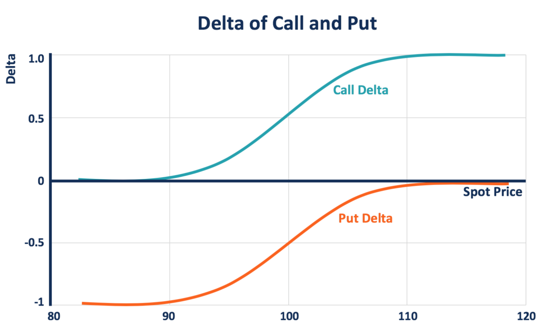
\includegraphics[scale=0.75]{../5-pictures/chapter-2_pic_1.png}
	\end{center}
\end{frame}
%..................................................................
\begin{frame}{Delta continued}
	\begin{itemize}
		\item Traders can make themselves delta-neutral by trading the underlying asset
		\item They also use delta as a measure of moneyness for call and put options
		\item Call is at-the-money when delta =0.5
		\item Call is in-the-money when delta > 0.5
		\item Call is out-of-the-money when delta < 0.5
		\item Put is at-the-money when delta = -0.5
		\item Put is in-the-money when delta <  -0.5
		\item Put is out-of-the-money when delta >  -0.5
	\end{itemize}
\end{frame}
%..................................................................
%=====================================================================


\end{document}

%..................................................................
\begin{frame}[fragile]
\frametitle{***}
\begin{itemize}
\item 
\end{itemize}
\rule{\textwidth}{1pt}
\scriptsize
\begin{minted}{python}

%python code

\end{minted}
\rule{\textwidth}{1pt}
\end{frame}
%..................................................................

%..................................................................
\begin{frame}{}
	\begin{itemize}
		\item ***
	\end{itemize}
\end{frame}
%..................................................................
